\chapter{Link--Discovery--System}
\label{system}

Das folgende Kapitel beschäftigt sich mit ausgewählten Aspekten der technischen Umsetzung der in \cref{link_discovery} beschriebenen Link--Discovery--Durchführung. Dazu gehören die Formulierung der Anforderungen an das System, die Systemarchitektur sowie die getroffene Technologieauswahl und einige Implementierungsaspekte.

\section{Anforderungen an das System}
\label{requirements}

Dieser Abschnitt spezifiziert die Anforderungen an ein System, das zur Link Discovery eingesetzt werden kann. Die Anforderungen unterteilen sich hierbei in einen funktionalen und einen nichtfunktionalen Anteil. 

\subsection{Funktionale Anforderungen}

Nachfolgend werden die funktionalen Anforderungen an das System aufgeführt. Diese ergeben sich direkt aus dem in \cref{ld_framework} beschriebenen Link--Discovery--Framework.

\paragraph{Datenimport} Das System muss in der Lage sein, Rohdaten aus verschiedenen Datenquellen zu importieren und zu speichern. Dazu zählen die MySQL--Datenbank des Unternehmens Spreadshirt, die JSON--Dokumente des Clicktracking--Systems und die API des Wortschatzes der Universität Leipzig. Das System sollte außerdem erweiterbar sein, um in Zukunft andere Datenquellen einbinden zu können.

\paragraph{Datenspeicherung} Das System muss die importierten Rohdaten, Zwischenergebnisse der Link Discovery und die Graphenrepräsentation des Weltausschnittes permanent speichern können.

\paragraph{Datenverarbeitung} Das System muss die importierten Daten entsprechend des in \cref{ld_process} beschriebenen Link--Discovery--Prozesses verarbeiten können. Dazu zählen die Schritte Bereinigung, Reduktion, Transformation und Integration. Die Implementierung dieser Schritte sollte änderbar und erweiterbar sein. Im Rahmen des Transformationsschrittes muss das System in der Lage sein, Kookkurrenzmaße zu berechnen.

\paragraph{Visualisierung} Das System soll eine Oberfläche für die Visualisierung der in der Graphenrepräsentation des Weltausschnittes gespeicherten Daten bieten. Dazu zählt einerseits die Darstellung der Begriffe, deren Kontext und Beziehungen und andererseits eine Möglichkeit der manuellen Priorisierung zum interaktiven Erkunden des Datenbestandes.

\paragraph{Priorisierung} Das System muss den in \cref{evo_for_prio} beschriebenen Priorisierungsprozess mittels evolutionärer Algorithmen implementieren. Dazu gehören Komponenten des Algorithmus aus \cref{evo_implementation} sowie eine Benutzeroberfläche zur interaktiven Selektion.

\paragraph{Programmierschnittstelle} Das System muss eine Programmierschnittstelle (nachfolgend \emph{API}) zur programmatischen Abfrage der Daten bereit stellen. Die angebotenen Daten enthalten die Begriffe, deren Kontexte und priorisierte Beziehungen. Die Priorisierung wird vom Benutzer der API spezifiziert.

\subsection{Nichtfunktionale Anforderungen}

Neben den funktionalen Anforderungen werden einige nichtfunktionale Anforderungen an das System gestellt. Diese werden im folgenden genannt.

\paragraph{Datenmenge} Das System muss in der Lage sein, bis zu einer Milliarde Objekte zu speichern und zu verarbeiten. Diese Objekte können Rohdaten der Datenquellen, Zwischenergebnisse der Link Discovery oder Knoten und Kanten des Weltausschnittes sein.

\paragraph{Parallelisierbarkeit} Um die Datenmenge verarbeiten zu können, sollten rechenintensive Berechnungsschritte auf mehrere Rechner verteilt werden können, um die Berechnung zu beschleunigen. Zu den anspruchsvolleren Berechnungsschritten zählt beispielsweise die Berechnung von Kookkurrenz aus den Daten des Tagging--Systems.

\paragraph{Antwortzeiten} Das System sollte Anfragen, die die Graphenrepräsentation des Weltausschnittes betreffen, in unter einer Sekunde beantworten. Hierzu zählt vor allem die Anfrage der Nachbarn eines Begriffes, geordnet nach einer spezifizierten Priorisierung.

Nachdem die Anforderungen an das System formuliert wurden, werden in den folgenden Abschnitten die sich daraus ergebende Architektur, das Datenmodell und die Technologieauswahl erläutert.

\section{Architektur des Systems}
\label{architecture}

Aus den im vorherigen Abschnitt formulierten Anforderungen wurde die im Folgenden beschriebene Systemarchitektur entwickelt. \cref{fig:architecture} zeigt die komplette Architektur des implementierten Link--Discovery--Systems. Darin sind, neben der Architektur des Systems selbst, alle genutzten Datenquellen und die Daten, die sie bereit stellen, aufgeführt.

\begin{figure}[t]
\centering
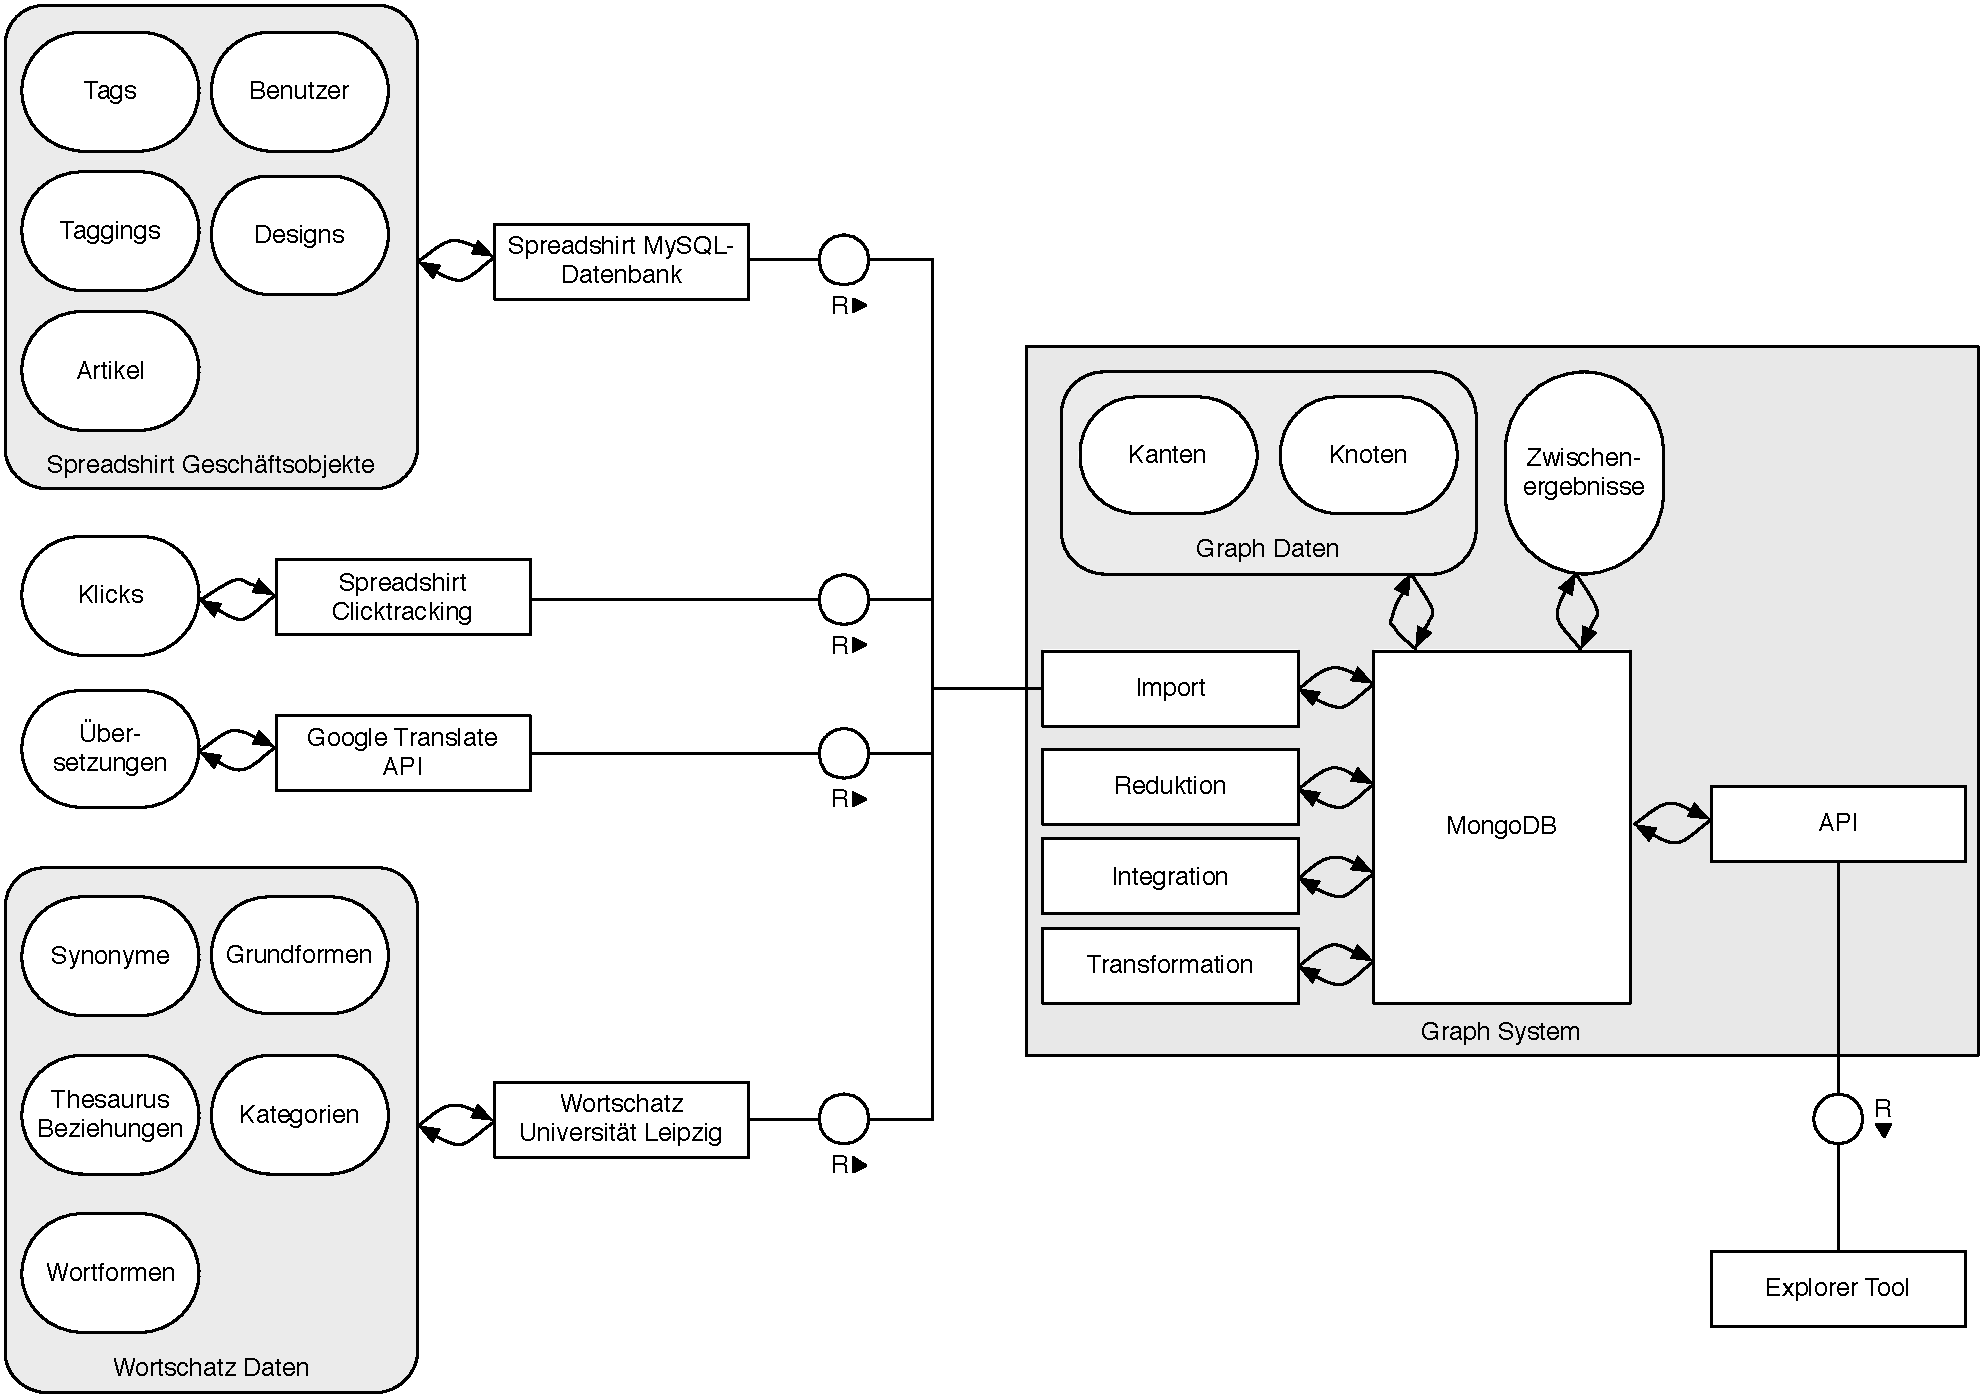
\includegraphics[width=1\textwidth]{architecture}
\caption{FMC--Blockdiagramm der gewählten Systemarchitektur}
\label{fig:architecture}
\end{figure}

Zentraler Bestandteil der Architektur ist das Datenbanksystem, das alle benötigten Daten speichert. Die Wahl des Datenbanksystems hat große Bedeutung für die Realisierung der funktionalen und nichtfunktionalen Anforderungen und wird in \cref{db_choice} diskutiert. Im Datenbanksystem werden die Rohdaten, Zwischenergebnisse und die Graphenrepräsentation des Weltausschnittes abgelegt. Das Datenmodell des Graphen folgt der Definition aus \cref{world_graph}.

Für jeden Schritt der Integration von Datenquellen aus \cref{integration_generic} existiert in der Architektur eine Komponente, die den jeweiligen Schritt für die entsprechende Datenquelle ausführt. Diese Komponenten kommunizieren direkt mit dem Datenbanksystem, um die Rohdaten oder Zwischenergebnisse zu lesen, führen die Berechnungen durch und speichern die Ergebnisse wiederum in die Datenbank.

Für die Abfrage der im Graphen gespeicherten Informationen existiert eine API, welche Informationen zu Knoten und deren Nachbarn per HTTP als JSON--Dokumente \cite{json2006} zur Verfügung stellt. Diese API kann für die Einbindung der erzeugten Informationen in andere Applikationen genutzt werden. Über Anfrageparameter kann die Gewichtung der einzelnen Kantentypen beeinflusst werden.

Zum Zeitpunkt der Bearbeitung dieser Arbeit existierten zwei Anwendungen, die die API des Link--Discovery--Systems nutzten. Dies sind der \emph{Tag Explorer} und die Komponente zur Priorisierung der Beziehungen.

Beim Tag Explorer handelt es sich um eine Browseranwendung, die die im Graphen gespeicherten Beziehungen visualisiert und interaktiv erkundbar macht. Der Benutzer dieser Anwendung kann mit selbst gewählten Gewichtungen der Beziehungen den Graphen durchsuchen. Außerdem werden, wenn vorhanden, die Designs auf der Spreadshirt--Plattform angezeigt, die mit dem gewählten Begriff getaggt sind. Somit wurde die funktionale Anforderung, den Kontext zu einem Begriff zu visualisieren, nur zum Teil umgesetzt, da der Tag Explorer lediglich den Tagging--Kontext eines Begriffes darstellt. In \cref{fig:tag_explorer} ist ein Screenshot der Anwendung abgebildet.

\begin{figure}[ht]
\centering
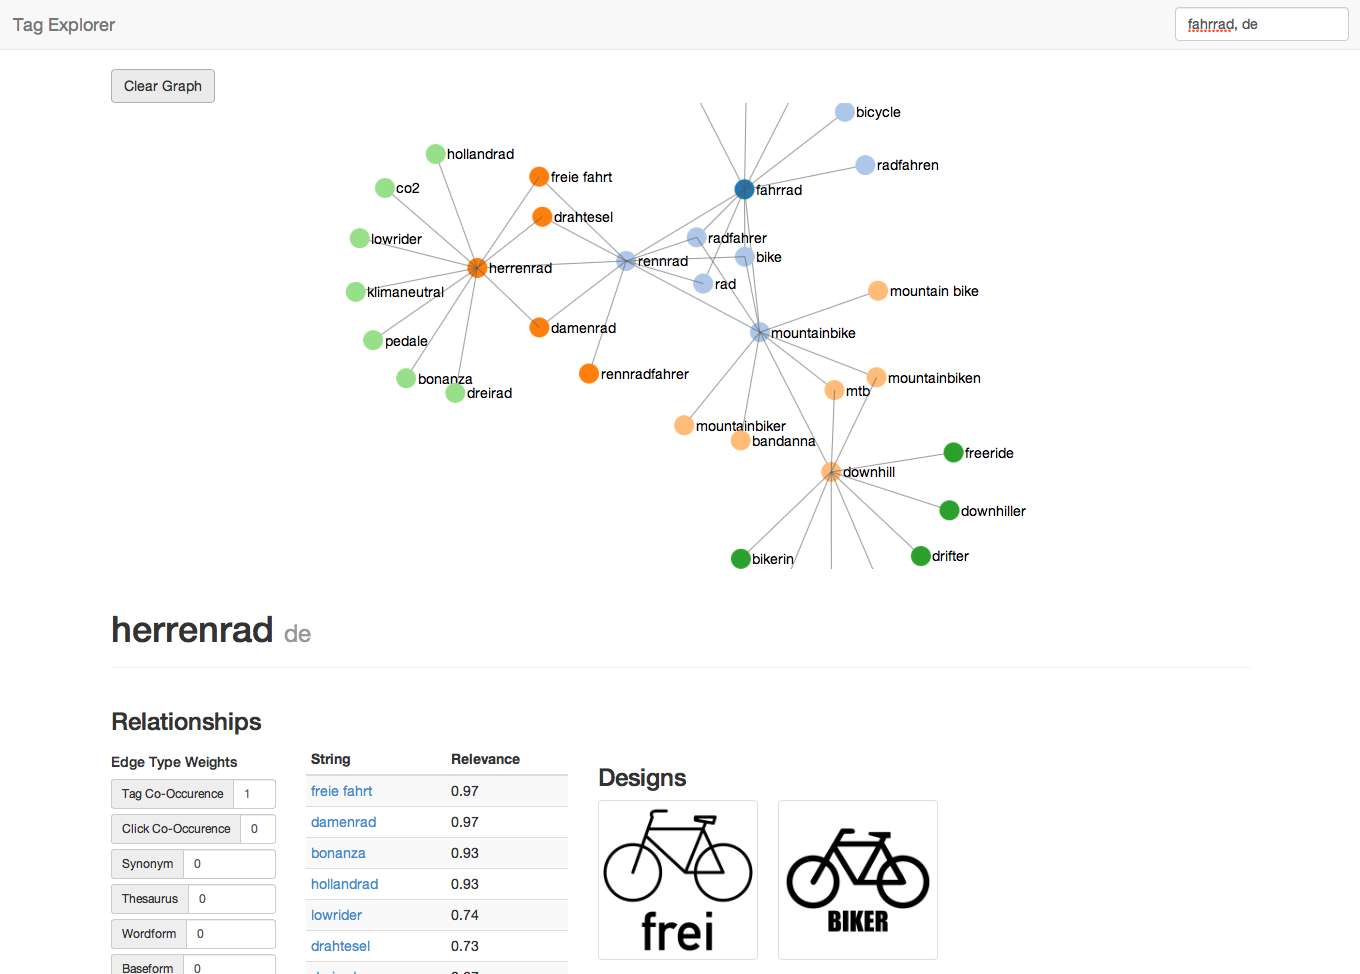
\includegraphics[width=\textwidth]{tag_explorer}
\caption{Screenshot der Anwendung ``Tag Explorer''}
\label{fig:tag_explorer}
\end{figure}

Die zweite Anwendung, die die API des Systems nutzt, ist die in \cref{evo_implementation} beschriebene Umsetzung der Priorisierung. Da diese die Daten des Weltausschnittes nicht verändern muss, ist eine entkoppelte Anbindung über die API sinnvoll.

Nachdem die Architektur vorgestellt wurde, spezifiziert der nächste Abschnitt die konkreten Technologien, die zur Implementierung dieser Architektur ausgewählt wurden.

\section{Technologieauswahl}
\label{tech}

Der folgende Abschnitt beschäftigt sich mit einer Auswahl der zur Umsetzung der Link Discovery eingesetzten Technologien. Die Kernelemente sind das Datenbanksystem, die konkrete Implementierung der Architekturkomponenten sowie die parallele Datenverarbeitung mittels des Programmiermodells MapReduce.

\subsection{Datenbanksystem}
\label{db_choice}

Die Wahl des Datenbanksystems ist von zentraler Bedeutung für die Umsetzung der in \cref{requirements} formulierten Anforderungen. Speziell die nichtfunktionalen Anforderungen der großen Datenmenge, der Parallelisierbarkeit und der kurzen Antwortzeiten stellen für traditionelle relationale Datenbanksysteme große Herausforderungen dar. Durch die starre relationale Form der Daten sind Schemaänderungen mit großem Aufwand verbunden. Die Verteilung von Daten über mehrere Server ist üblicherweise nicht grundsätzlich vorgesehen und kann nur mit größerem Implementierungsaufwand erreicht werden. Aufgrund dieser häufigen Limitierungen relationaler Datenbanksysteme wurde für die Implementierung des Link--Discovery--Systems das Datenbanksystem \emph{MongoDB} \cite{mo2013} gewählt.

\subsubsection{MongoDB}
\label{mongo}

Bei MongoDB handelt es sich um eine quelloffene dokumentenorientierte Datenbank. Im Gegensatz zu traditionellen relationalen Datenbanksystemen verzichtet MongoDB auf eine tabellenförmige Struktur der Daten und speichert Datensätze in Form von so genannten \emph{Dokumenten}. Dabei handelt es sich um hierarchische Schlüssel-/Wertpaare, die schemalos in so genannten \emph{Collections} gespeichert werden. Schemalos bedeutet, dass die Dokumente innerhalb einer Collection nicht alle dieselbe Struktur besitzen müssen.

Zur Repräsentation der Dokumente verwendet MongoDB ein Format, das sich sehr an JSON \cite{json2006} anlehnt. JSON ist ein menschenlesbares Datenaustauschformat, das aus der Objektnotation der Programmiersprache JavaScript abgeleitet wurde. Das Datenformat von MongoDB ist BSON \cite{bson2013}, eine binäre Repräsentation von JSON, die einige zusätzliche Datentypen unterstützt. 

\begin{lstlisting}[language=json, label={lst:json}, caption={JSON--Beispiel für ein Dokument in MongoDB}, float=ht]
{
    "_id" : ObjectId("51efc20147cae77dfc02e0ac"),
    "name" : "Bob",
    "age": 25,
    "address": {
        "city": "Leipzig",
        "street": "Karl--Liebknecht--Str. 132"
        "zip": "04277"
    },
    "friends" : [
        "alice",
        "fred",
        "jason"
    ]
}
\end{lstlisting}

\cref{lst:json} zeigt ein Beispiel für ein Dokument in MongoDB. Das Feld \emph{\_id} ist hierbei ein  Bezeichner vom Typ \emph{ObjectID}. Dieser stellt einen global eindeutigen Bezeichner dar, der benutzt werden kann, um Dokumente zu referenzieren. Innerhalb einer Collection muss \emph{\_id} grundsätzlich eindeutig sein. Das Feld \emph{address} zeigt, dass Dokumente weitere Dokumente enthalten können. Am Feld \emph{friends} wird deutlich, dass Werte für Schlüssel auch Arrays von Werten sein können. Diese sind nicht auf primitive Typen wie Zeichenketten oder Zahlen beschränkt, sondern können auch weitere Dokumente oder Arrays sein.

MongoDB unterstützt Anfragen über ein Binärprotokoll, welches über so genannte \emph{Treiber} in vielen Programmiersprachen abstrahiert zur Verfügung steht. Dieses Protokoll unterstützt vielfältige Lese- und Schreiboperationen, die komplexe Abfragen und Operationen auf den gespeicherten Daten zulassen. Außerdem bietet MongoDB eine Implementierung des MapReduce--Programmiermodells (siehe \cref{mapreduce}) sowie die Möglichkeit, Indizes auf allen Hierarchieebenen der Dokumente zu nutzen. Für interaktive Operationen steht die \emph{Mongo Shell} zur Verfügung, welche Abfragen mittels der Programmiersprache JavaScript erlaubt und somit einen Treiber für diese Sprache darstellt.

Aufgrund der genannten Eigenschaften stellt MongoDB einen exzellenten Ausgangspunkt für die Link Discovery im Rahmen dieser Arbeit dar. Durch die vorhandene Schemaflexibilität können die Daten in der gerade benötigten Form gespeichert und abgefragt werden. Durch die Unterstützung von MapReduce mit mehreren Rechnern lassen sich Berechnungen wie die der Kookkurrenz (siehe \cref{mapreduce_cooccurence}) parallelisieren und somit beschleunigen. Die Unterstützung von Indizes auf allen Hierarchieebenen der Dokumente bietet Vorteile zur effektiven Verkürzung von Antwortzeiten auf Anfragen.

MongoDB stellt das zentrale technische Element für die Link Discovery im Rahmen dieser Arbeit dar. Sobald die Daten aus den externen und internen Quellen in MongoDB importiert wurden, können die folgenden Schritte direkt mit Datenbankabfragen realisiert werden.

\clearpage

\subsubsection{Umsetzung der Graphenrepräsentation}

Um das in \cref{world_graph} beschriebene Datenmodell in MongoDB umzusetzen, muss es in eine Dokumentenform überführt werden. Dazu bietet es sich an, Knoten in Kanten in unterschiedlichen Collections zu speichern, um sie voneinander zu trennen.

Somit stellt sich anschließend die Frage, wie die Knoten und Kanten als Dokumente repräsentiert werden. Durch die durch MongoDB gegebene Schemaflexibilität lassen sich die Kontexte der durch die Knoten repräsentierten Begriffe direkt als Unterdokumente im Knotendokument ablegen. Der Schlüssel für diese Unterdokumente ist der Name des Kontextes. Dadurch lassen sich die Knoten leicht filtern, da die Abfrage auf das Vorhandensein des jeweiligen Schlüssels angepasst und durch Indizes auf diesen Schlüsseln unterstützt werden kann. \cref{lst:node_json} zeigt ein Beispiel für einen Knoten in JSON--Notation. Arrays mit vielen Elementen sind aus Platzgründen verkürzt dargestellt.

\begin{lstlisting}[language=json, label={lst:node_json}, caption={JSON--Beispiel für ein Knotendokument in MongoDB}, float=ht]
{
    "_id" : ObjectId("51efc22447cae77dfc03e16b"),
    "language" : "de",
    "string" : "segeln",
    "tagProperties" : {
        "occurenceCount" : 4678,
        "articleCount" : 2347,
        "designCount" : 2331,
        "articleIDs" : [ 
            4961057, 
            4977725, 
            ...
        ],
        "designIDs" : [ 
            1645572, 
            2216059, 
            ...
        ]
    },
    "wortschatzProperties" : {
        "synonyms" : [ 
            "flattern", 
            "fliegen", 
            "gaukeln", 
            ...
        ]
    }
}
\end{lstlisting}

Die Kanten können direkt als Dokumente abgebildet werden. Über den Typ ergeben sich zusätzliche Eigenschaften. Ein Kantendokument für eine Tagging--Kookkurrenz ist beispielhaft in  \cref{lst:edge_json} dargestellt.

\begin{lstlisting}[language=json, label={lst:edge_json}, caption={JSON--Beispiel für ein Kantendokument}, float=ht]
{
        "_id" : ObjectId("51efd6f61177ff360605bd99"),
        "source" : ObjectId("51efc1af47cae77dfc00c3f8"),
        "target" : ObjectId("51efc1e047cae77dfc02087c"),
        "type" : "tag-co-occurence",
        "occurences" : 1,
        "dice" : 0.0001317089232795522,
        "jaccard" : 0.00006585879873551106,
        "cosine" : 0.008115343414514944
}
\end{lstlisting}

\subsection{Implementierung der Komponenten der Architektur}
\label{arch_components_impl}

Die Komponenten zum Import, zur Bereinigung, Reduktion, Transformation und Integration wurden in der Programmiersprache JavaScript als Skripte für die Mongo Shell (siehe \cref{mongo}) umgesetzt. Diese Skripte implementieren die funktionalen Anforderungen an das System.

JavaScript wurde ausgewählt, da die Sprache eine natürliche Interaktion mit dem JSON--Format ermöglicht. Die Mongo Shell stellt alle Operationen für MongoDB für diese Programmiersprache zur Verfügung und eignet sich damit gut zur Kommunikation mit dem Datenbanksystem.

Die API wurde ebenfalls in JavaScript programmiert, unter Zuhilfenahme der Laufzeitumgebung \emph{node.js} \cite{node}. Diese ermöglicht die serverseitige Benutzung von JavaScript und ist demnach gut geeignet, um mit den Daten aus MongoDB zu arbeiten und diese als JSON--Dokumente an Clients auszuliefern. Der Tag Explorer sowie die Oberfläche zur interaktiven Selektion sind in JavaScript als Browseranwendungen implementiert.

Einzig die Importskripte für die MySQL--Datenbank von Spreadshirt und den Wortschatz der Universität Leipzig wurden in der Programmiersprache Ruby umgesetzt, da diese zum Zeitpunkt des Imports bessere Unterstützung für diese Datenquellen bot.

Zusammenfassend lässt sich festhalten, dass die Architekturkomponenten größtenteils als Skripte implementiert wurden, die direkt mit MongoDB kommunizieren. Dadurch kann das System bei Benutzung von weiteren Datenquellen einfach erweitert werden.

\clearpage

\subsection{Datenverarbeitung}
\label{mapreduce}

Um die nichtfunktionalen Anforderungen an das Link--Discovery--System umzusetzen, wurde zur Verarbeitung der Daten, speziell zur Kookkurrenzberechnung, das Programmiermodell MapReduce gewählt, da dieses die parallele Verarbeitung großer Datenmengen ermöglicht. Die Grundlagen dieses Modells sowie die Umsetzung der Kookkurrenzberechnung werden in den folgenden Abschnitten beschrieben.

\subsubsection{Grundlagen von MapReduce}
\label{mapreduce_basic}

MapReduce \cite{dg2004} ist ein Programmiermodell für nebenläufige Verarbeitung und Erzeugung großer Datenmengen. Der Grundgedanke dieses Modells besteht in der Zerlegung der Berechnung in zwei Funktionen: \emph{Map} und \emph{Reduce}. Die Ein- und Ausgabedaten sind Schlüssel-/Wertpaare. Beide Funktionen werden vom Benutzer spezifiziert.

Die Map--Funktion dient zur Erzeugung von Zwischenergebnissen, welche ebenfalls in der Form von Schlüssel-/Wertpaaren vorliegen. Die Funktion wird einzeln auf jedes Paar der Eingabedaten angewandt und kann eine beliebige Anzahl von Zwischenergebnissen \emph{emittieren}. Die MapReduce--Bibliothek gruppiert daraufhin alle Paare mit dem gleichen Schlüssel und übergibt diese an die Reduce--Funktion.

Die Reduce--Funktion wird somit jeweils auf einen Schlüssel und eine Liste von Werten angewandt. Ziel dieser Funktion ist, für jeden Schlüssel kein oder ein Ergebnis zurückzugeben. Die zu reduzierenden Werte werden für gewöhnlich als Iterator übergeben, um auch Datenmengen verarbeiten zu können, die nicht in den Arbeitsspeicher des Rechenknotens passen. Die Reduce--Funktion wird nur angewandt, wenn nach dem Map--Schritt mehr als ein Wert für einen Schlüssel emittiert wurde. Somit sollten Map- und Reduce--Funktion das gleiche Ausgabeformat besitzen. Das grundsätzliche Vorgehen von MapReduce ist in \cref{fig:mapreduce} abgebildet.

\begin{figure}
\centering
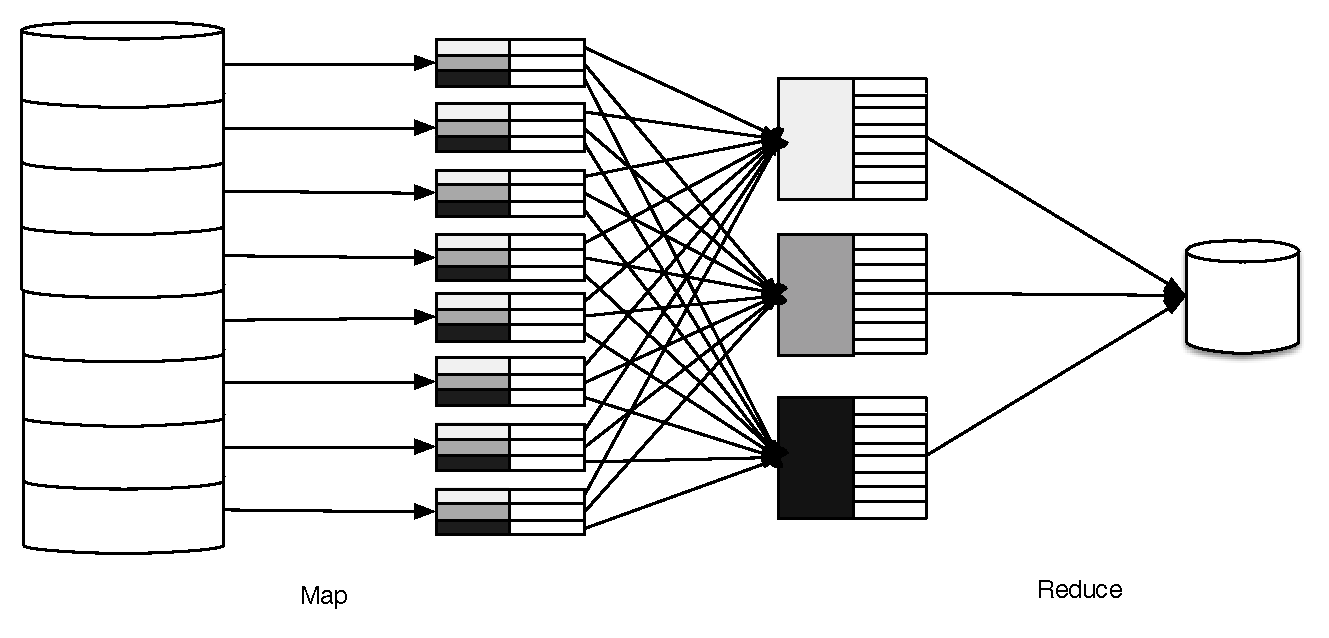
\includegraphics[width=\textwidth]{mapreduce}
\caption{MapReduce--Prozess}
\label{fig:mapreduce}
\end{figure}

Die MapReduce--Bibliothek übernimmt die Kommunikation zwischen den Knoten des Rechnerclusters. Dies hat den Vorteil, dass sich der Programmierer nur über die Umwandlung des zu lösenden Problems auf das Programmiermodell, nicht aber um dessen Implementierung über mehrere Rechner hinweg kümmern muss. Somit kann die verwendete Hardware vergleichsweise einfach an die zu verarbeitende Datenmenge oder die Bedürfnisse an die Rechengeschwindigkeit angepasst werden.

In dieser Arbeit wurde die MapReduce Implementierung von MongoDB eingesetzt (siehe \cref{db_choice}).

\subsubsection{Kookkurrenzberechnung mit MapReduce}
\label{mapreduce_cooccurence}

MapReduce kann für die Berechnung der Knoten und Kanten mittels Kookkurrenz genutzt werden. Dazu müssen für beide Operationen das Ein- und Ausgabeformat sowie die Funktionen Map und Reduce definiert werden.

Um die Berechnung zu vereinfachen, werden zuerst die Knoten erzeugt und mit allen Vorkommen der Begriffe annotiert. Somit kann daraufhin direkt aus der Knotenmenge die Kantenmenge erzeugt werden. Außerdem werden bei der Nutzung der Daten weniger Anfragen benötigt, um Informationen über einen Begriff selbst zu bekommen.

\paragraph{Berechnung der Knoten}

Als Eingabedaten für die Berechnung der Knotenmenge dienen Tupel der Form \((d, t)\), wobei \(d\) ein Dokument und \(t\) einen Begriff darstellt. Die Map--Funktion wird nun auf jeden dieser Tupel angewandt und emittiert Schlüssel-/Wertpaare mit dem Begriff als Schlüssel und einer einelementigen Liste, die das Dokument des Tupels enthält sowie der Zahl \num{1} als Anzahl Vorkommen dieses Begriffs. Dieses Vorgehen ist notwendig, da die Ausgabe der Map- und Reduce--Funktionen das gleiche Datenformat haben sollten.

Die Reduce--Funktion fasst die einelementigen Listen zusammen, addiert die Vorkommen und erzeugt somit den Knoten, der für einen Begriff alle Dokumente, die mit diesem Begriff versehen wurden, sowie die Anzahl der Vorkommen insgesamt enthält.

Die Map- und Reduce--Funktionen für die Knotenberechnung sind als Pseudo--Code in \cref{lst:mapred_nodes} dargestellt.

\begin{lstlisting}[language=pseudo, label={lst:mapred_nodes}, caption={Knotenerzeugung mit MapReduce}, float]
function map(document, term) {
    emit(term, {documents: [document], count: 1});
}

function reduce(term, values) {
    result = {documents: [], count: 0};
    foreach value in values do
        result.documents = concat(result.documents, value.documents);
        result.count = result.count + value.count;
    end
    return result;
}
\end{lstlisting}

\paragraph{Berechnung der Kanten}

Die Berechnung der Kantenmenge kann mit den vorher berechneten Knoten als Eingabedaten erfolgen und wird in 2 Verarbeitungsschritte aufgeteilt. Zuerst werden die annotierten Knoten so umgeformt, dass zu einem Dokument alle vergebenen Begriffe bekannt sind. Im zweiten Schritt werden alle Paare von miteinander auftretenden Begriffen gebildet und die Ähnlichkeitsmaße berechnet.

\cref{lst:mapred_edges1} zeigt die Umformung der Knoten mittels MapReduce. Als Eingabe für die Map--Funktion dienen die Knoten. Diese werden so umgeformt, dass für jedes Dokument, das am Knoten annotiert ist, ein neues Schlüssel-/Wertpaar emittiert wird. Die emittierten Ergebnisse werden in der Reduce--Funktion zusammengefasst, so dass als Ergebnis alle Begriffe, die an ein Dokument vergeben wurden, gesammelt als Liste vorliegen.

\begin{lstlisting}[language=pseudo, label={lst:mapred_edges1}, caption={Umformung der Knoten mit MapReduce}, float=ht]
function map(node) {
    foreach document in node.documents do
        emit(document, {terms: [node]});
    end
}

function reduce(term, values) {
    result = {terms: []};
    foreach value in values do
        result.terms = concat(result.terms, value.terms);
    end
    return result;
}
\end{lstlisting}

In \cref{lst:mapred_edges2} wird die Erzeugung der Kookkurrenzkanten dargestellt. Im Map--Schritt werden dazu alle möglichen Paare der mit einem Dokument verknüpften Begriffe gebildet und emittiert. Der Schlüssel ist eine Kombination aus Ziel- und Quellbegriff. Der Wert zählt die Anzahl der Kookkurrenzen zwischen beiden Begriffen. Während des Reduce--Schrittes werden alle Kanten zwischen zwei Begriffen zusammengefasst, die Summe der Kookkurrenzen gebildet und die Ähnlichkeitsmaße berechnet. Die Funktionen zur Berechnung der Maße sind in \cref{measures} beschrieben.

\begin{lstlisting}[language=pseudo, label={lst:mapred_edges2}, caption={Kantenerzeugung mit MapReduce}, float=ht]
function map(document) {
    foreach term1 in document.terms do
        foreach term2 in document.terms do
            emit({source: term1, target: term2}, {count: 1});
        end
    end
}

function reduce(edge, values) {
    result = {count: 0, dice: 0, jaccard: 0, cosine: 0};
    foreach value in values do
        result.count = result.count + value.count;
    end
    result.dice = dice(edge.source, edge.target, result.count);
    result.jaccard = jaccard(edge.source, edge.target, result.count);
    result.cosine = cosine(edge.source, edge.target, result.count);
    return result;
}
\end{lstlisting}

MapReduce eignet sich somit gut zur Beschleunigung der Kookkurrenzberechnung, da diese in drei Schritten ohne sequenzielle Anteile auf die Funktionen Map und Reduce abgebildet werden kann, wie in diesem Abschnitt gezeigt wurde.

\section{Zusammenfassung}

Dieses Kapitel beschäftigte sich mit den Implementierungsaspekten des Systems, welches für die in \cref{link_discovery} beschriebene Link--Discovery--Durchführung im Rahmen dieser Arbeit zum Einsatz kam. Dazu wurden die funktionalen und nichtfunktionalen Anforderungen an das System formuliert. Aus diesen Anforderungen und dem Prozess zur Link Discovery aus \cref{ld_process} wurde eine Architektur für das System abgeleitet und erläutert. Abschließend wurden einige Technologien, die zur Implementierung des Systems zum Einsatz kamen, diskutiert. Hierzu gehören MongoDB als Datenbanksystem, JavaScript als Sprache für die einzelnen Komponenten der Systemarchitektur und MapReduce als übergeordnetes Programmiermodell sowie dessen konkreter Einsatz zur Kookkurrenzberechnung.